% Created 2018-10-26 vie 00:10
% Intended LaTeX compiler: pdflatex
\documentclass[xcolor={usenames,svgnames,dvipsnames}]{beamer}
\usepackage[utf8]{inputenc}
\usepackage[T1]{fontenc}
\usepackage{graphicx}
\usepackage{grffile}
\usepackage{longtable}
\usepackage{wrapfig}
\usepackage{rotating}
\usepackage[normalem]{ulem}
\usepackage{amsmath}
\usepackage{textcomp}
\usepackage{amssymb}
\usepackage{capt-of}
\usepackage{hyperref}
\usepackage{color}
\usepackage{listings}
\usepackage{mathpazo}
\usepackage{gensymb}
\usepackage{amsmath}
\usepackage{chemarr}%flechas para reacciones químicas (SFER.tex)
\bibliographystyle{plain}
\AtBeginSubsection[]{\begin{frame}[plain]\tableofcontents[currentsubsection,sectionstyle=show/shaded,subsectionstyle=show/shaded/hide]\end{frame}}
\AtBeginSection[]{\begin{frame}[plain]\tableofcontents[currentsection,hideallsubsections]\end{frame}}
\usepackage[emulate=units]{siunitx}
\sisetup{fraction=nice, decimalsymbol=comma, retain-unity-mantissa = false}
\newunit{\wattpeak}{Wp}
\newunit{\watthour}{Wh}
\newunit{\amperehour}{Ah}
\usepackage{steinmetz}
\hypersetup{colorlinks=true, linkcolor=Blue, urlcolor=Blue}
\renewcommand{\thefootnote}{\fnsymbol{footnote}}
\beamertemplatenavigationsymbolsempty
\setbeamertemplate{footline}[frame number]
\setbeamercolor{alerted text}{fg=blue!50!black} \setbeamerfont{alerted text}{series=\bfseries}
\usetheme[hideothersubsections]{Goettingen}
\usecolortheme{rose}
\usefonttheme{serif}
\author{Oscar Perpiñán Lamigueiro}
\date{\url{http://oscarperpinan.github.io}}
\title{Máquinas Eléctricas \\ Aparamenta Eléctrica}
\hypersetup{
 pdfauthor={Oscar Perpiñán Lamigueiro},
 pdftitle={Máquinas Eléctricas \\ Aparamenta Eléctrica},
 pdfkeywords={},
 pdfsubject={},
 pdfcreator={Emacs 25.2.2 (Org mode 9.1.13)}, 
 pdflang={Spanish}}
\begin{document}

\maketitle

\section{Fundamentos de Electromagnetismo}
\label{sec:orge24c6d5}

\begin{frame}[label={sec:org127a0f0}]{Fuerza Magnética}
Un campo magnético ejerce una fuerza sobre una carga en movimiento (o corriente eléctrica en un conductor) \footnote{Fuerza de Lorentz}.
\[
\vec{F} = q (\vec{v} \times \vec{B})
\]

\begin{columns}
\begin{column}{0.5\columnwidth}
\begin{center}
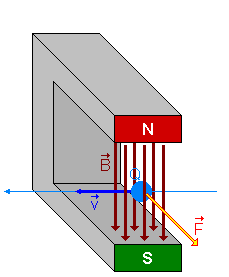
\includegraphics[height=0.5\textheight]{../figs/Fuerza_Lorentz.png}
\end{center}
\end{column}

\begin{column}{0.5\columnwidth}
\begin{center}
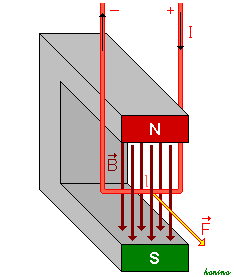
\includegraphics[height=0.5\textheight]{../figs/Fuerza_Lorentz_Conductor.png}
\end{center}
\end{column}
\end{columns}
\end{frame}

\begin{frame}[label={sec:org91a048f}]{Campo Magnético creado por un Conductor}
Una corriente eléctrica crea un campo magnético en torno al conductor\footnote{Ley de Biot-Savart (y Oersted). Ley de Ampere.}. 

\begin{columns}
\begin{column}{0.5\columnwidth}
\begin{center}
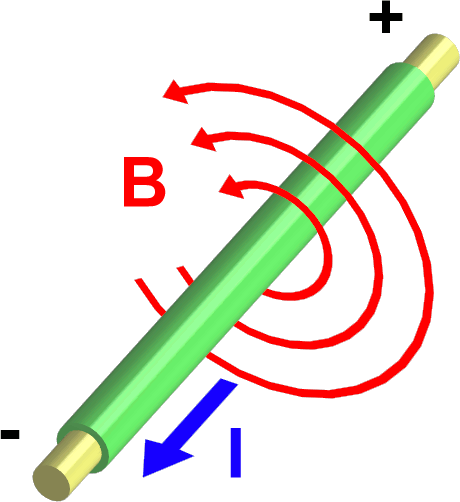
\includegraphics[width=.9\linewidth]{../figs/Electromagnetism.png}
\end{center}
\end{column}
\begin{column}{0.5\columnwidth}
\begin{center}
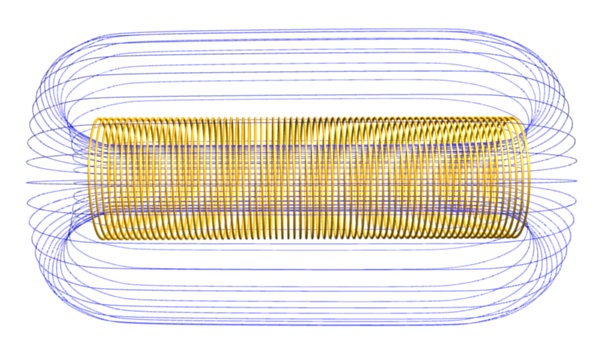
\includegraphics[width=.9\linewidth]{../figs/Solenoide.jpg}
\end{center}
\end{column}
\end{columns}
\end{frame}

\begin{frame}[label={sec:orge8dab45}]{Interacción entre Conductores}
Dos conductores se repelen o atraen según el sentido de sus corrientes.

\begin{center}
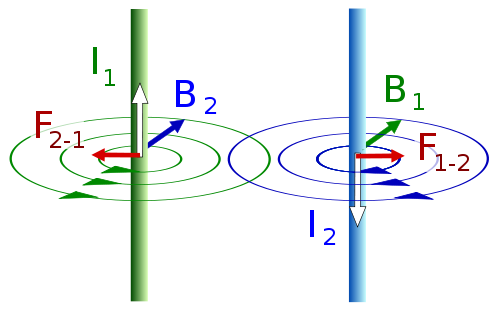
\includegraphics[width=.9\linewidth]{../figs/FuerzasRepulsion.png}
\end{center}
\begin{center}
Vídeo: \href{https://www.youtube.com/watch?v=2j8D\_N1v0tU\&t=0m15s}{Repulsión entre barras de Alta Tensión}
\end{center}
\end{frame}
\begin{frame}[label={sec:orgcd5ab30}]{Flujo Magnético}
El flujo magnético es la cantidad de líneas de fuerza magnética que atraviesan una superficie. 

Depende de la densidad de campo, \(B\), el área de la superficie, \(A\), y la posición relativa entre ambos, \(\theta\).

\[
\phi = B \cdot A \cdot \cos \theta
\]

\begin{center}
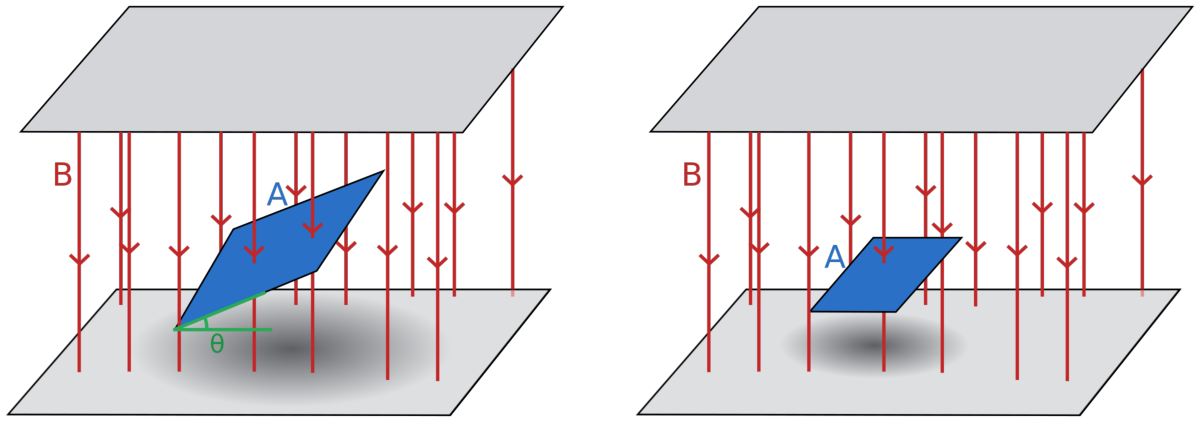
\includegraphics[width=.9\linewidth]{../figs/flujo_magnetico.pdf}
\end{center}
\end{frame}

\begin{frame}[label={sec:org8732474}]{Ley de Faraday}
\begin{itemize}
\item Cuando el \alert{flujo magnético} que atraviesa una espira es \alert{variable}
aparece \alert{tensión inducida}.
\end{itemize}

\[
e=- N \frac{\mathrm{d}\phi}{\mathrm{d}t} = - N \frac{\mathrm{d}(B \cdot S\cdot \cos \theta)}{\mathrm{d}t} 
\]

\begin{itemize}
\item El flujo es variable cuando:

\begin{itemize}
\item La \alert{espira está en movimiento} (\(\theta\))

\item El \alert{campo magnético \(B\) es variable},

\item Ambas situaciones coinciden.
\end{itemize}

\item La tensión inducida es directamente proporcional a la rapidez de la
variación.
\end{itemize}
\end{frame}


\section{Máquinas Eléctricas}
\label{sec:org42cecca}
\subsection{Introducción}
\label{sec:org399a8eb}

\begin{frame}[label={sec:org4e47adc}]{Máquina Eléctrica}
Una máquina eléctrica realiza una conversión entre dos formas de energía, una de ellas eléctrica:

\begin{itemize}
\item \alert{Motor}: transforma la energía eléctrica en energía mecánica.
\item \alert{Generador}: transforma la energía mecánica en energía eléctrica.
\item \alert{Transformador}: transforma las condiciones (tensión y corriente) de la energía eléctrica de entrada en otras diferentes de salida.
\end{itemize}
\end{frame}

\begin{frame}[label={sec:orgf93eb53}]{Partes de una Máquina}
\begin{columns}
\begin{column}{0.5\columnwidth}
\begin{itemize}
\item \alert{Estátor}: parte fija de forma cilíndrica.
\item \alert{Rótor}: parte giratoria situada en la cavidad del estátor.
\item \alert{Entrehierro}: espacio de aire que separa el estátor del rótor.
\end{itemize}
\end{column}
\begin{column}{0.5\columnwidth}
\begin{center}
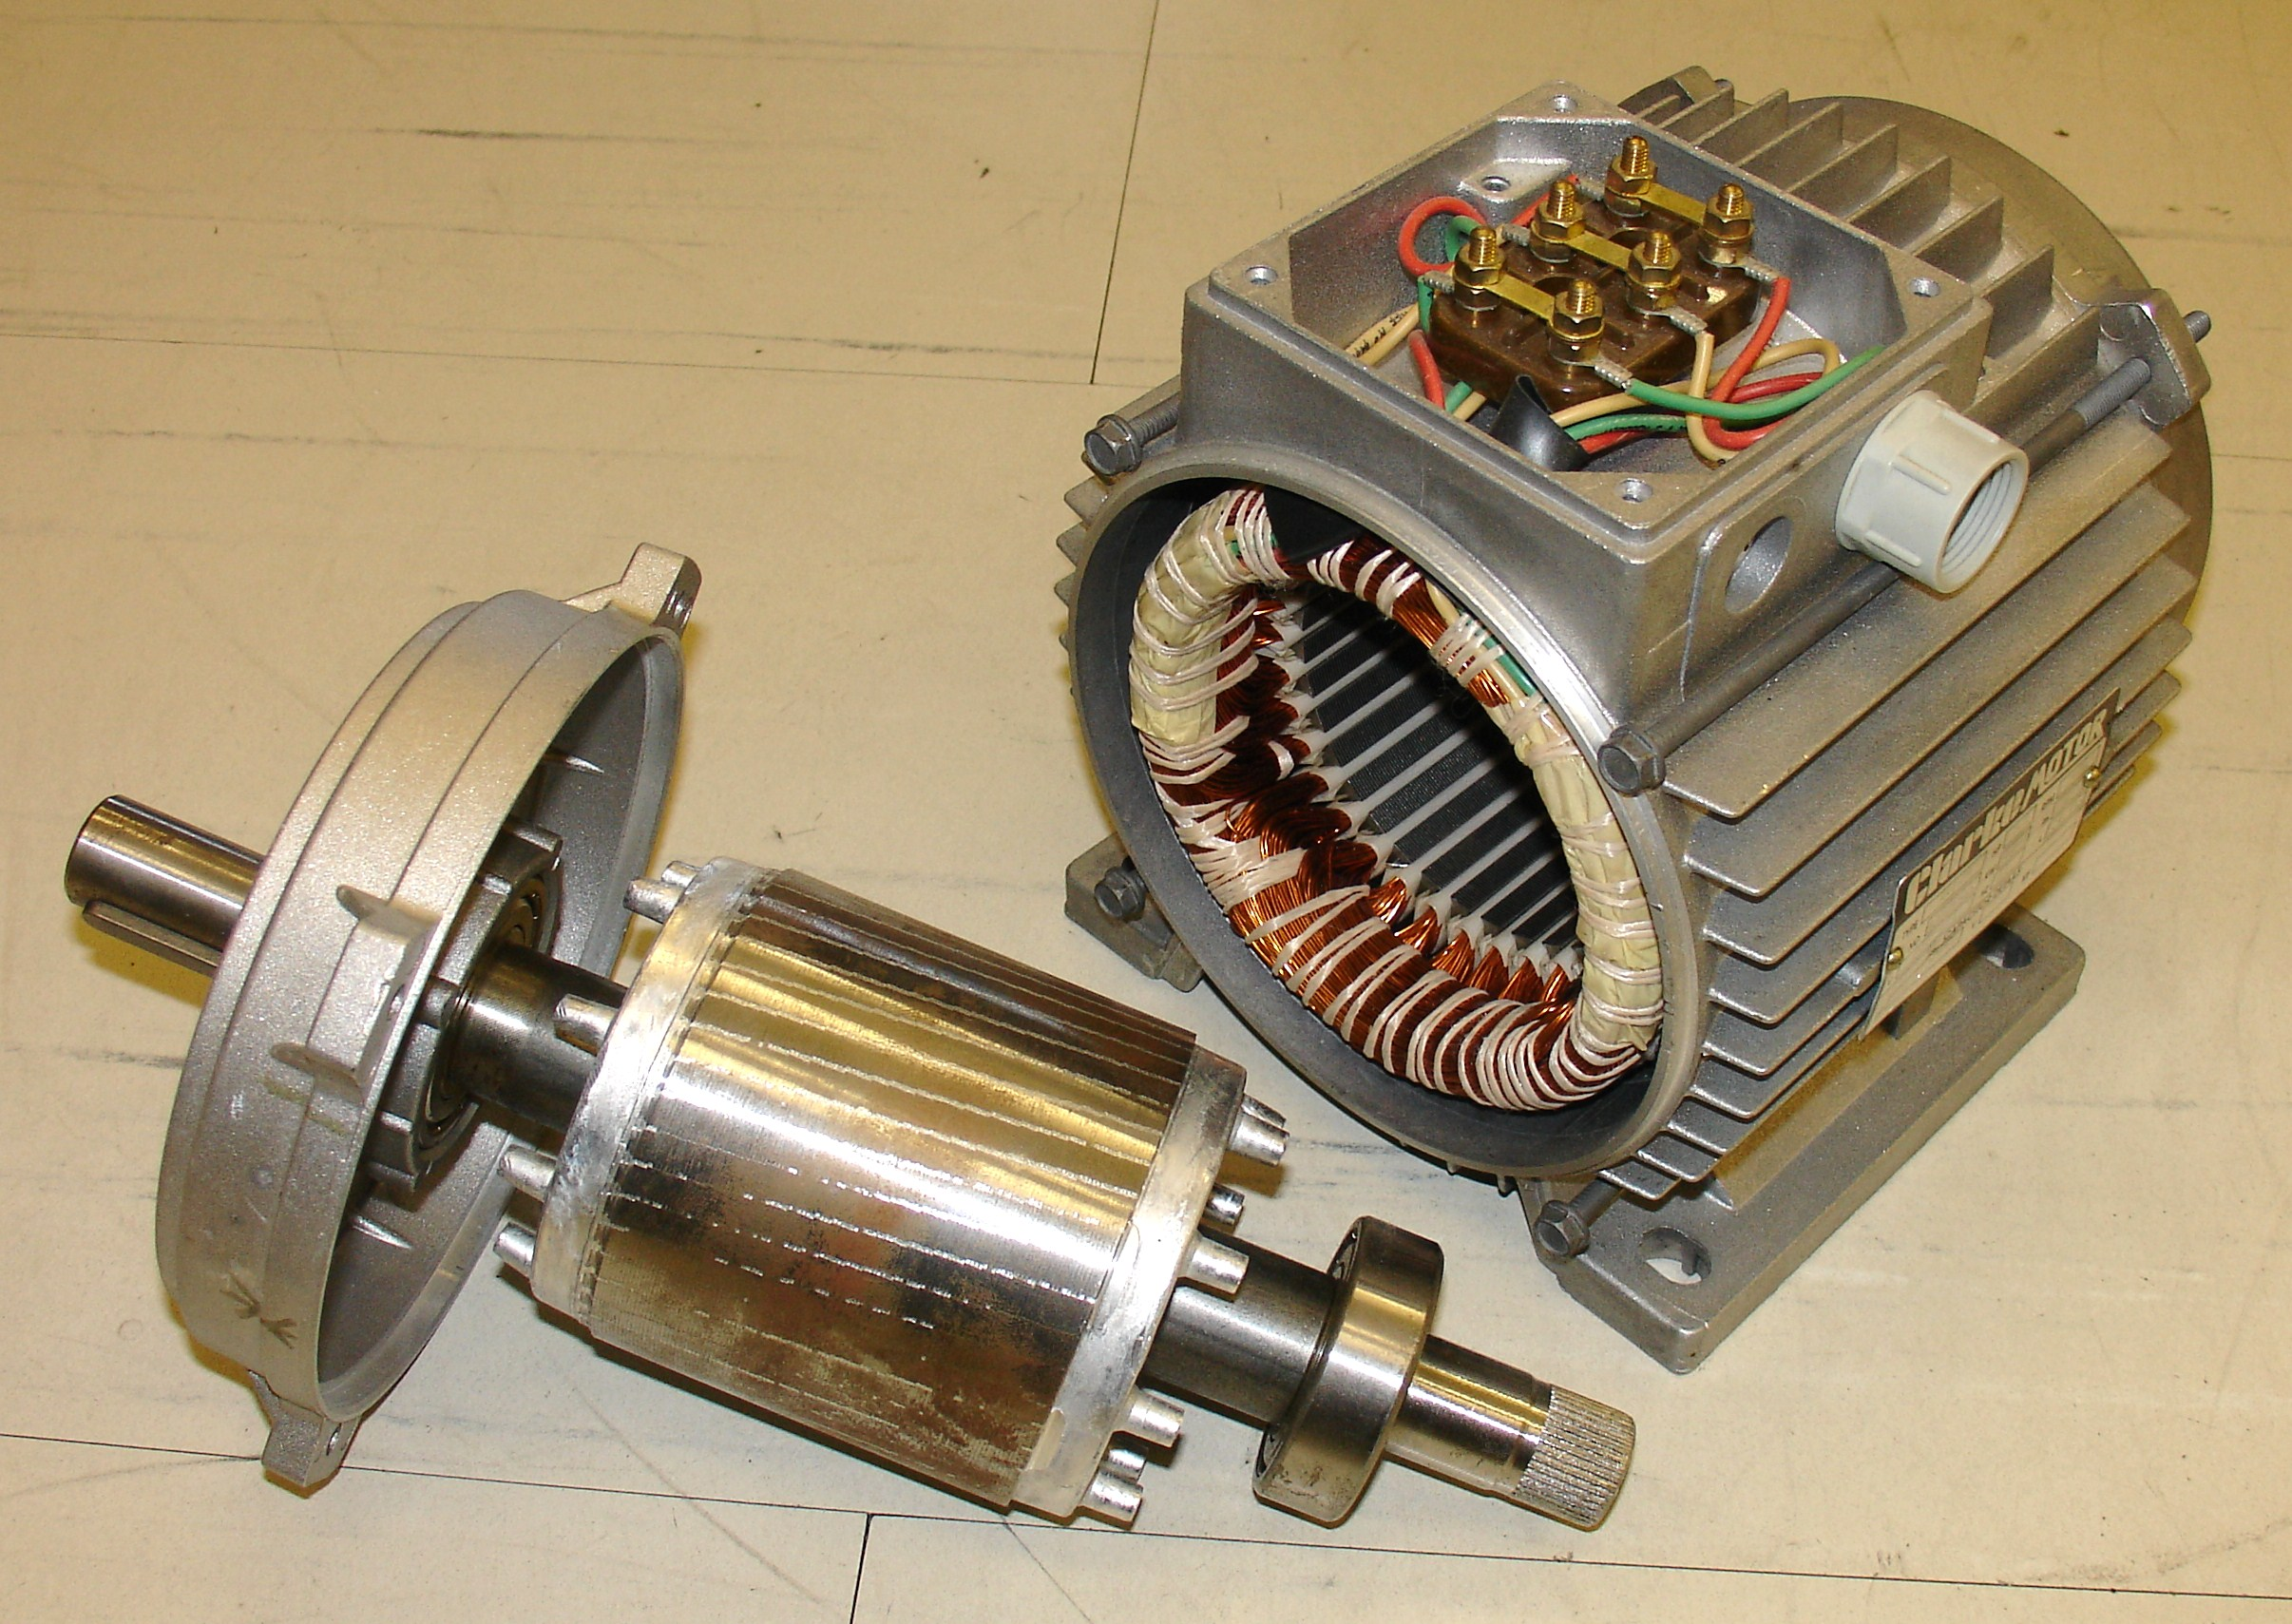
\includegraphics[width=.9\linewidth]{../figs/Stator_and_rotor_by_Zureks.jpeg}
\end{center}
\end{column}
\end{columns}

\begin{block}{}
La transformación de energía eléctrica y mecánica se produce a través del campo magnético del entrehierro, lugar del acoplamiento energético entre estátor y rótor. 
\end{block}
\end{frame}

\begin{frame}[label={sec:org9931e6d}]{Inductor e Inducido}
Al elemento que emite el campo magnético se le denomina \alert{inductor} y aquel que es atravesado por este flujo es el \alert{inducido}.
\begin{center}
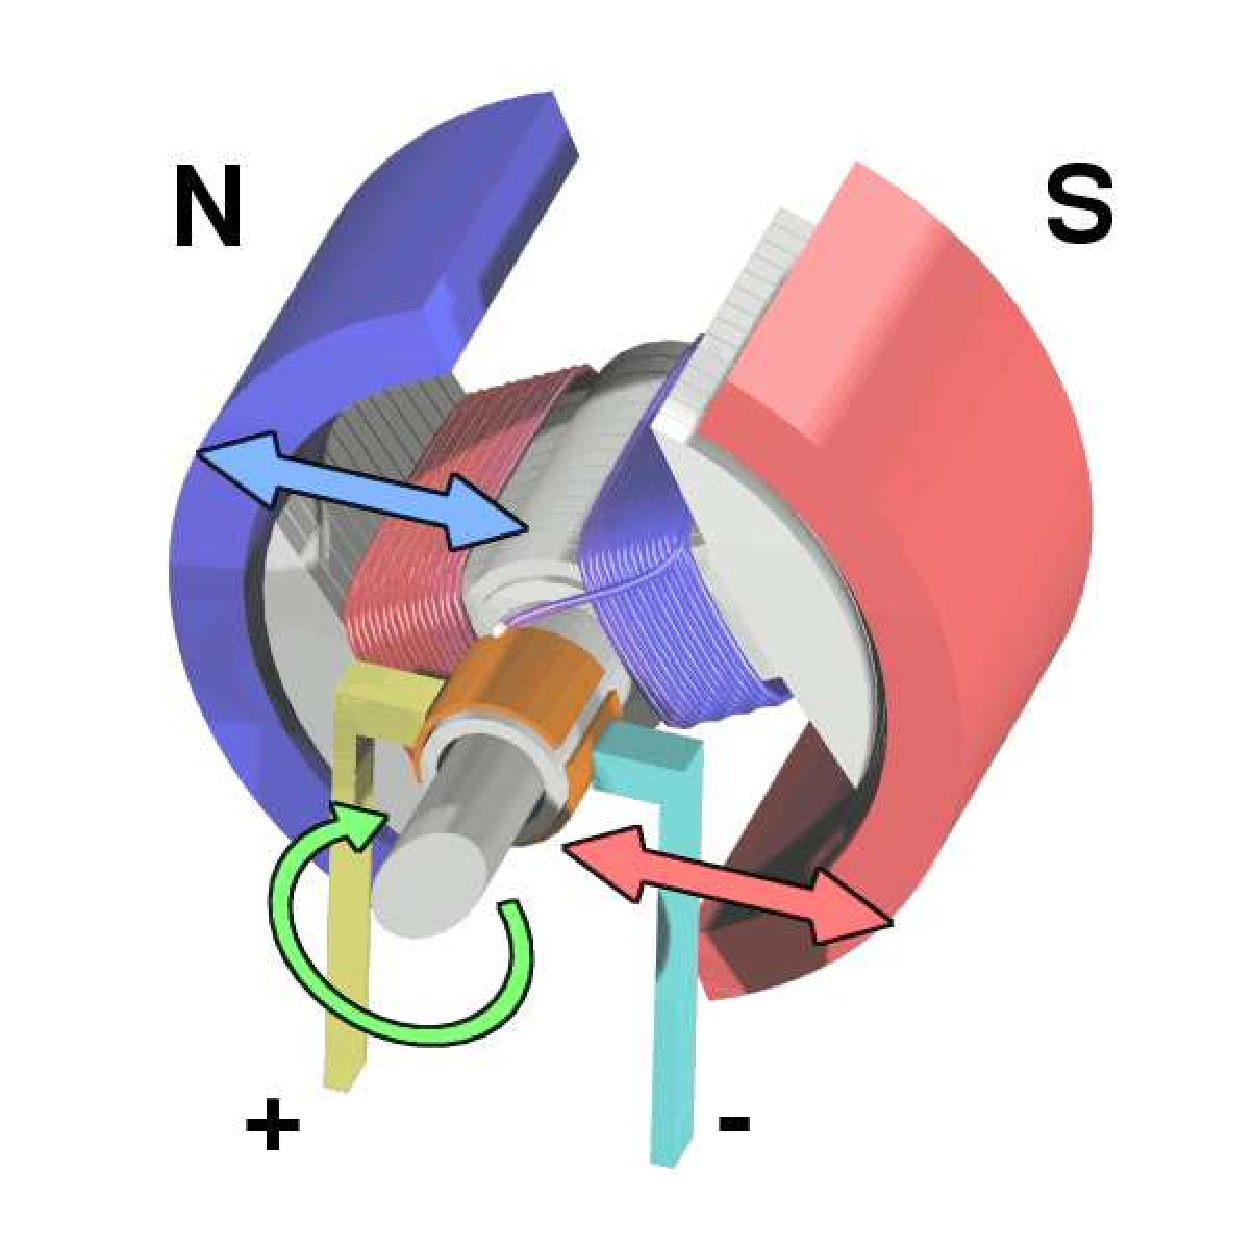
\includegraphics[height=0.5\textheight]{../figs/Electric_motor_cycle_3.pdf}
\end{center}
\end{frame}

\subsection{Motor}
\label{sec:orgcf07c78}
\begin{frame}[label={sec:org5bf2508}]{Fundamento}
\begin{itemize}
\item La energía eléctrica de \alert{entrada} produce una \alert{corriente eléctrica} que genera un \alert{campo magnético variable}.
\item Este campo puede \alert{interactuar} con otro \alert{campo magnético existente} o con \alert{otro conductor}, y produce movimiento.
\item Más habituales:
\begin{itemize}
\item \emph{Inducción}
\item \emph{Corriente Continua}.
\end{itemize}
\end{itemize}
\end{frame}


\begin{frame}[label={sec:orgdb691ba}]{Motor asíncrono o de inducción}
\begin{itemize}
\item \alert{Estator-Inductor} alimentado por una \alert{corriente trifásica alterna} (\emph{campo giratorio})

\item \alert{Rotor-Inducido} constituido por espiras cortocircuitadas (\alert{jaula de ardilla}).

\item Rotor gira a menor velocidad que el campo.
\end{itemize}

\begin{center}
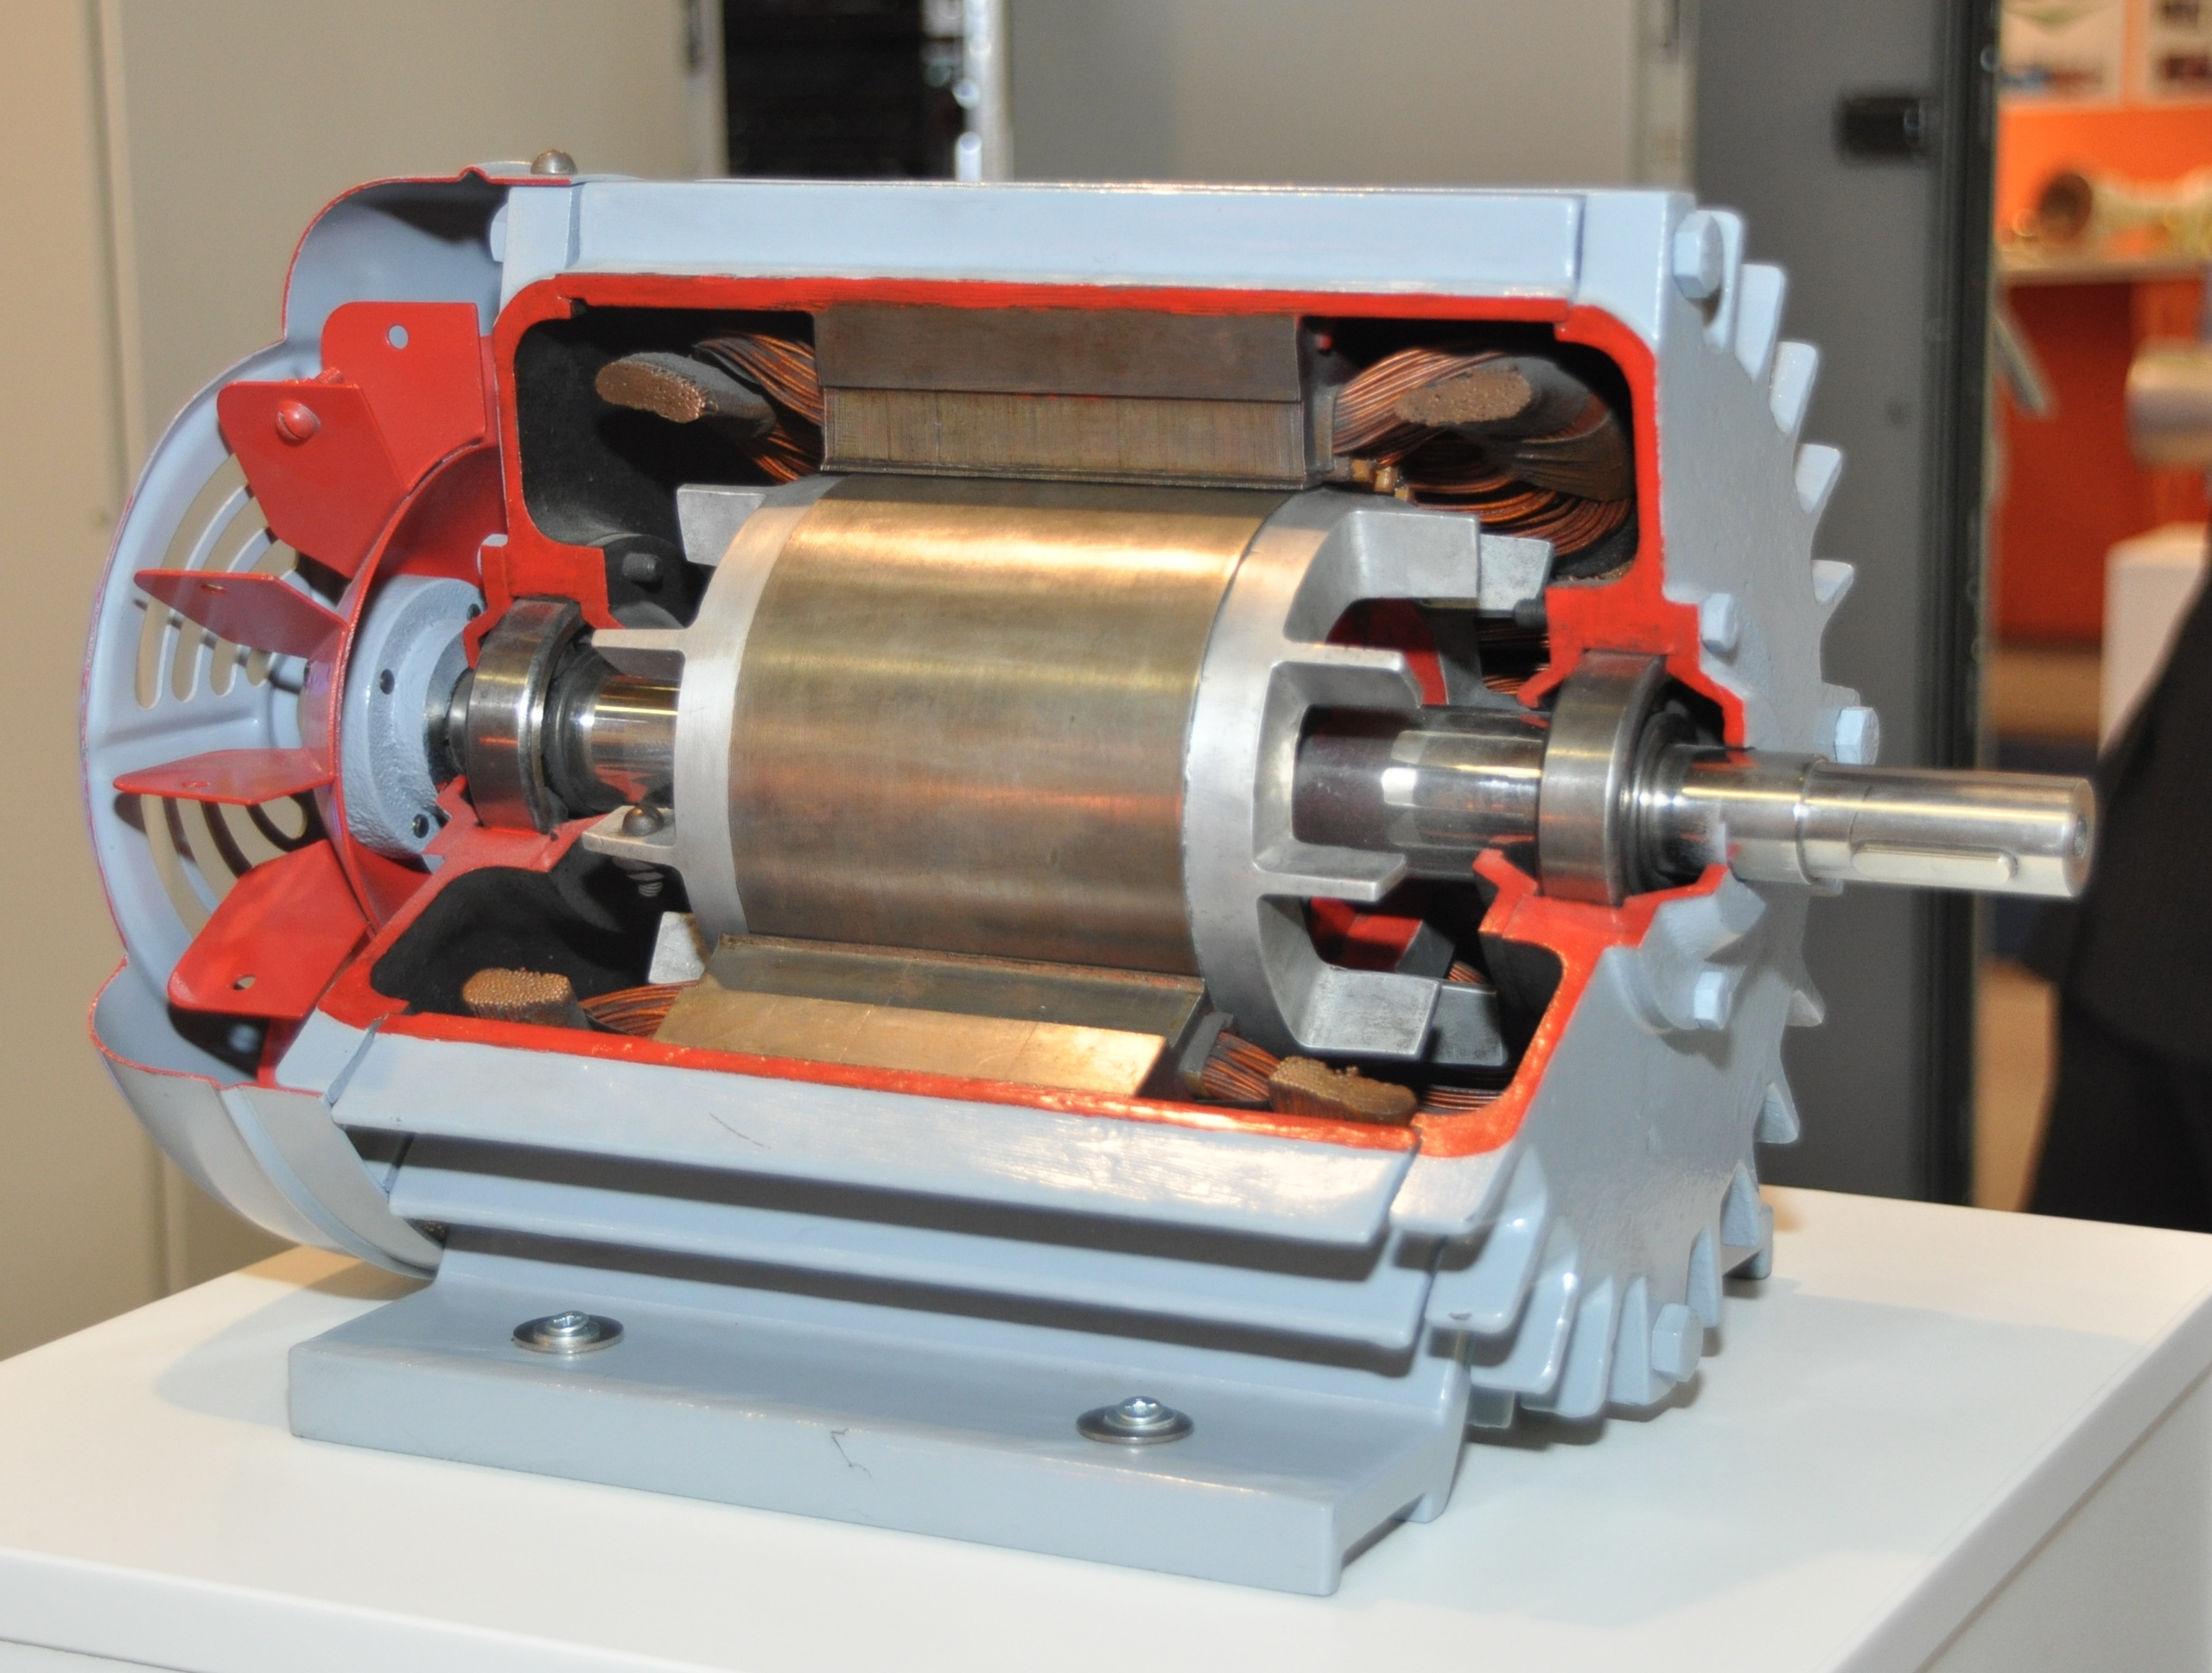
\includegraphics[height=0.5\textheight]{../figs/Seccion_Motor.jpeg}
\end{center}

Vídeos: Motor de inducción artesanal \href{http://www.youtube.com/watch?v=ZRGlAu0uCHY\&feature=related}{(1)} \href{http://www.youtube.com/watch?v=P-eTLmJC2cQ}{(2)}
\end{frame}

\begin{frame}[label={sec:orgcb46dce}]{Motor DC}
\begin{itemize}
\item \alert{Estator-Inductor} genera \alert{campo constante} (imanes permanentes o alimentado por corriente DC).

\item \alert{Rotor-Inducido} alimentado con \alert{corriente DC} a través de un colector de delgas, o sin escobillas.
\end{itemize}

\begin{center}
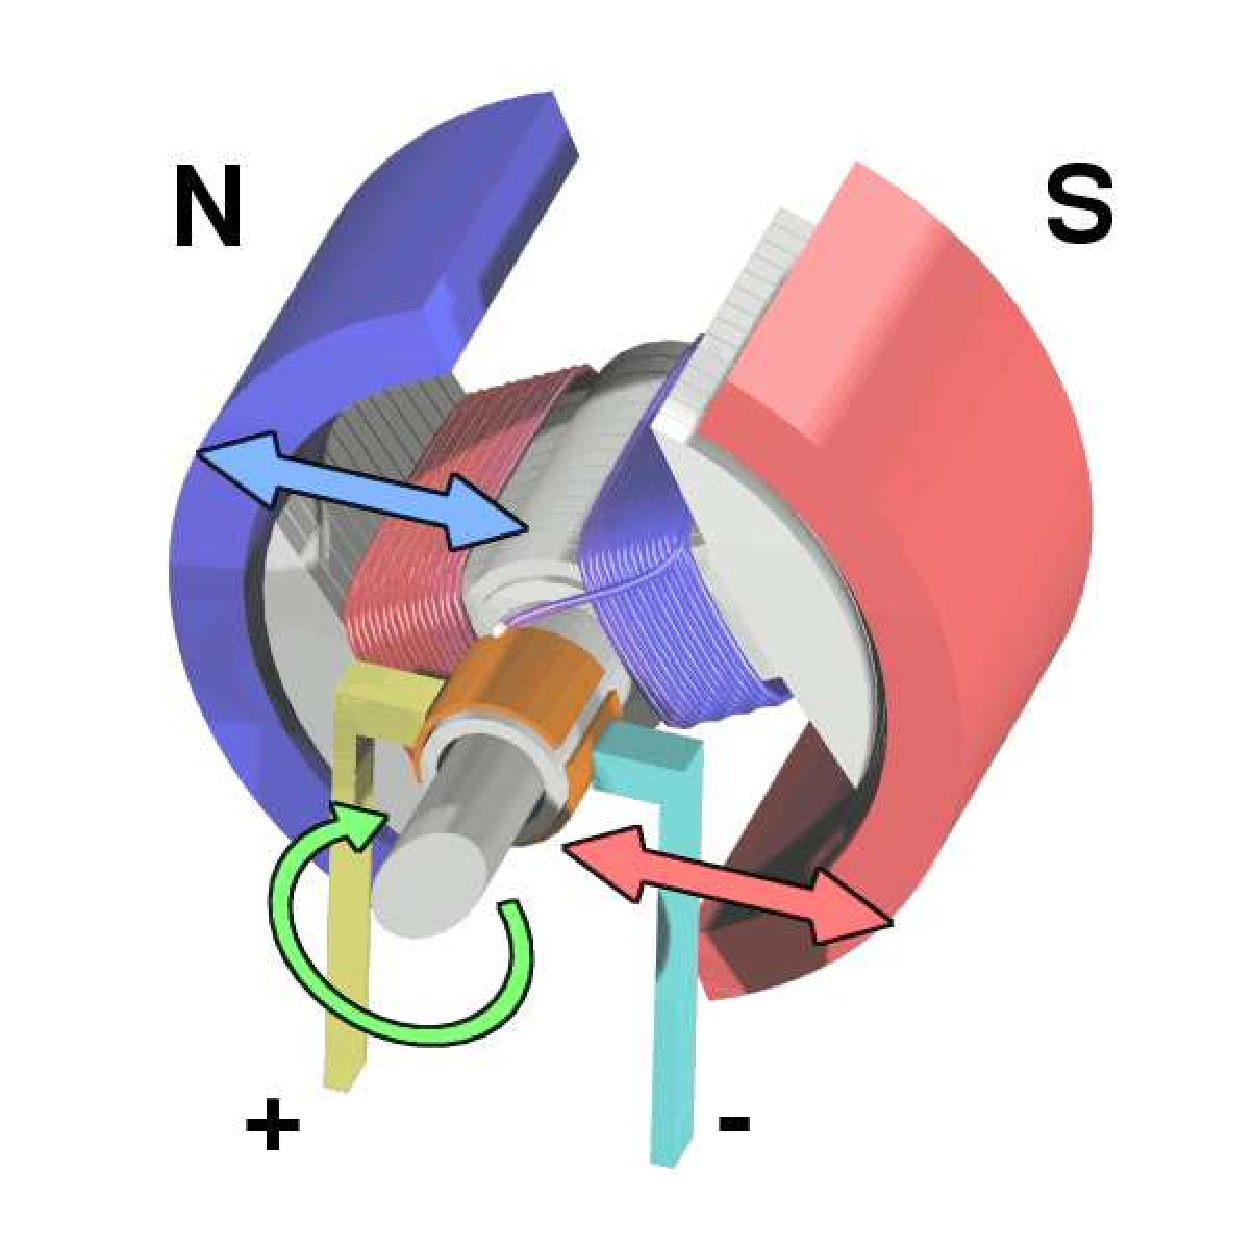
\includegraphics[height=0.6\textheight]{../figs/Electric_motor_cycle_3.pdf}
\end{center}
\end{frame}


\subsection{Generador}
\label{sec:orge3efac1}

\begin{frame}[label={sec:org4c0d458}]{Fundamento}
\begin{itemize}
\item Existe un \alert{campo magnético en el interior de la máquina} (p. ej. imanes permanentes)
\item La \alert{energía mecánica de entrada} aporta \alert{movimiento a una bobina} en el seno del campo.
\item La \alert{interacción} entre el campo y las espiras de la bobina producen una \alert{tensión inducida}.
\item Más habituales:
\begin{itemize}
\item \emph{Síncrono}
\item \emph{Asíncrono}
\item \emph{Corriente Continua}.
\end{itemize}
\end{itemize}
\end{frame}


\begin{frame}[label={sec:orgb405b27}]{Generador Síncrono o Alternador}
\begin{itemize}
\item \alert{Rotor-inductor} alimentado por \alert{corriente continua} mediante anillos.

\item \alert{Estator-inducido} constituido por un \alert{devanado trifásico}.

\item Velocidad de giro constante, sincronizada con la frecuencia de red.

\item Empleado en turbinas hidráulicas y térmicas.
\end{itemize}
\end{frame}

\begin{frame}[label={sec:org1566632}]{Generador Asíncrono}
\begin{columns}
\begin{column}{0.6\columnwidth}
\begin{itemize}
\item \alert{Estator} alimentado por una corriente trifásica (\emph{campo giratorio}).

\item \alert{Rotor} constituido por espiras cortocircuitadas (\alert{jaula de ardilla}).

\item Si el rotor gira a mayor velocidad que el campo del estator, se induce corriente \guillemotleft{}de vuelta\guillemotright{} en el estator.

\item Empleado en turbinas eólicas.
\end{itemize}
\end{column}

\begin{column}{0.5\columnwidth}
\begin{center}
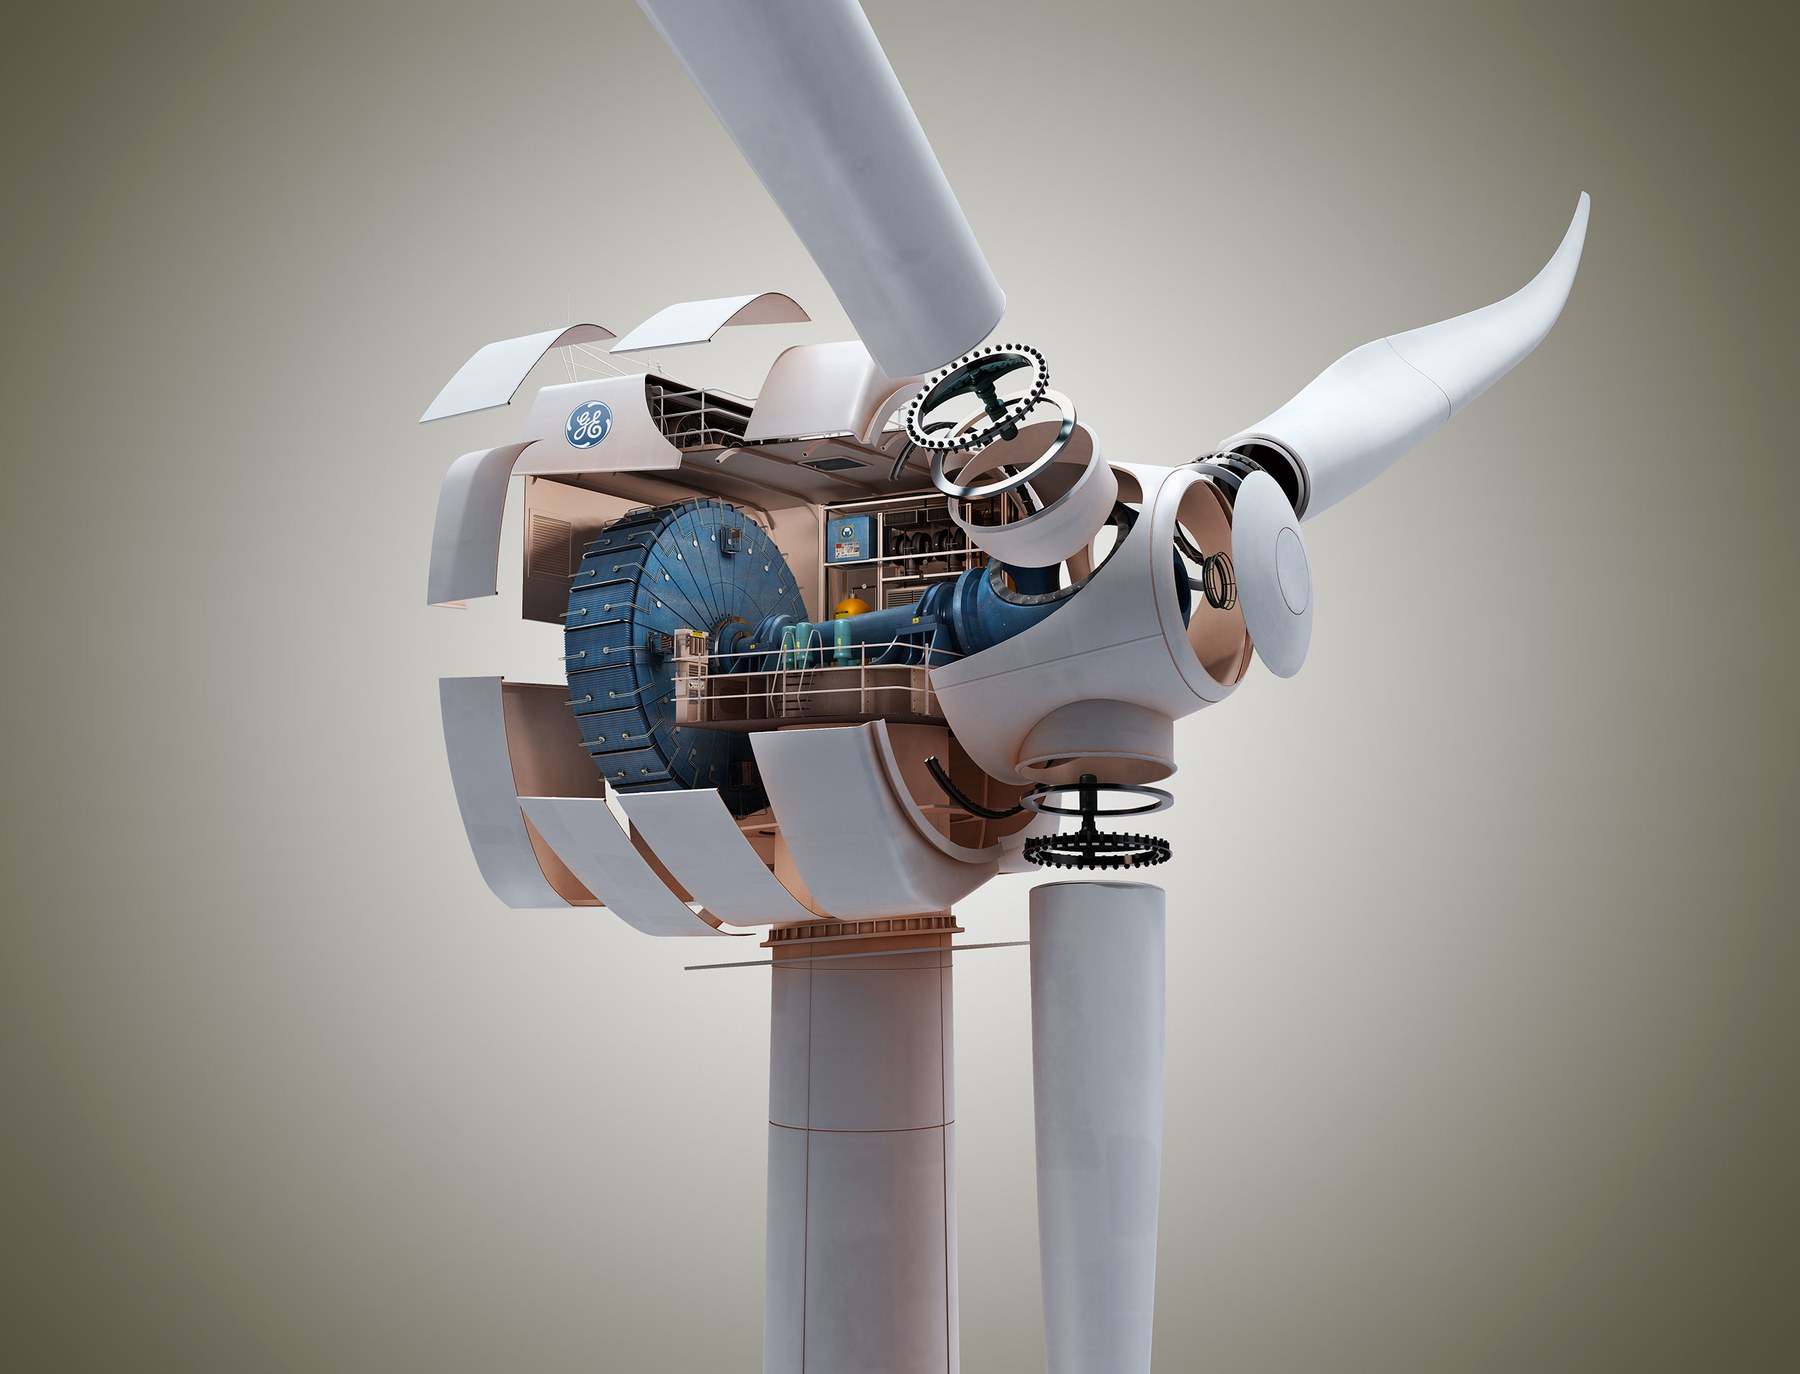
\includegraphics[width=.9\linewidth]{../figs/InsideWindTurbine.jpg}
\end{center}
\end{column}
\end{columns}
\end{frame}

\begin{frame}[label={sec:orgff89faa}]{Generador DC}
\begin{itemize}
\item \alert{Estator-Inductor} genera campo constante (alimentado por corriente DC o imanes permanentes).

\item El movimiento aplicado en el \alert{Rotor-Inducido} en el seno del campo produce una \alert{tensión inducida}.

\item El colector de delgas transforma alterna en continua.

\item Empleado en máquinas eólicas de baja potencia.
\end{itemize}
\end{frame}


\subsection{Transformador}
\label{sec:org52536ef}
\begin{frame}[label={sec:org6ba17bb}]{Fundamento}
\begin{columns}
\begin{column}{0.6\columnwidth}
\begin{itemize}
\item La energía eléctrica de entrada alimenta una bobina con un número de espiras \(N_p\).
\item El campo magnético generado por esta bobina circula hasta una bobina de salida, con \(N_s\) espiras.
\item El diferente número de espiras provoca valores de tensión y corriente diferente en la entrada y salida.
\end{itemize}
\end{column}

\begin{column}{0.4\columnwidth}
\begin{center}
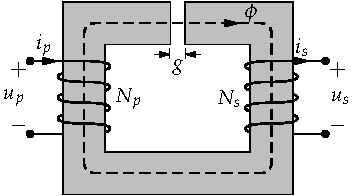
\includegraphics[width=.9\linewidth]{../figs/Transformador2.pdf}
\end{center}
\begin{center}
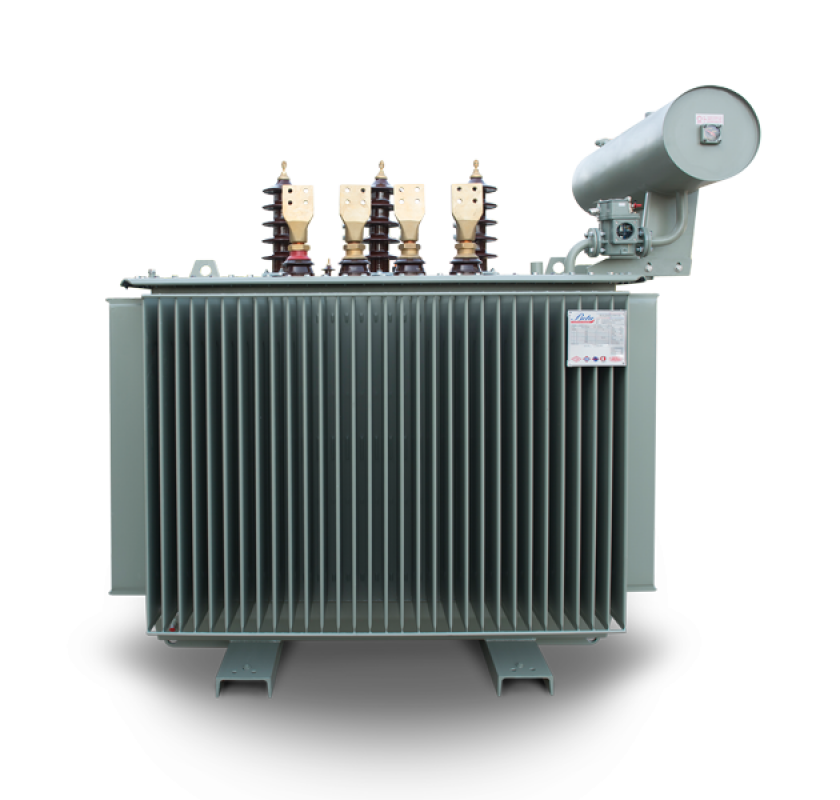
\includegraphics[width=.9\linewidth]{../figs/Transformador.png}
\end{center}
\end{column}
\end{columns}
\end{frame}

\begin{frame}[label={sec:org10c790b}]{Relación de Transformación}
\begin{align*}
N_{s}\cdot I_{s} &= N_{p}\cdot I_{p}\\
\frac{V_{p}}{N_{p}} &= \frac{V_{s}}{N_{s}}
\end{align*}

\begin{center}
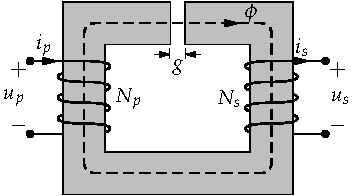
\includegraphics[height=0.3\textheight]{../figs/Transformador2.pdf}
\end{center}

\begin{itemize}
\item Ejemplo: un transformador elevador sube tensión (\(V_{s}>V_{p}\)) y reduce corriente (\(I_{s}<I_{p}\)): \(N_{p}/N_{s}<1\), más vueltas en el secundario que en el primario.
\end{itemize}
\end{frame}


\section{Aparamenta eléctrica}
\label{sec:org45f386a}

\subsection{Sistema de Suministro Eléctrico}
\label{sec:orgc090299}
\begin{frame}[label={sec:orgd86ce4f}]{Sistema de suministro eléctrico}
Un \alert{sistema de suministro eléctrico} tiene como objetivo \alert{producir,
transportar y distribuir energía eléctrica} a los lugares de consumo,
con el mínimo coste posible en condiciones de \alert{fiabilidad, calidad y
seguridad}.
\end{frame}

\begin{frame}[label={sec:org37a337f}]{Componentes del Sistema de Suministro Eléctrico}
\begin{center}
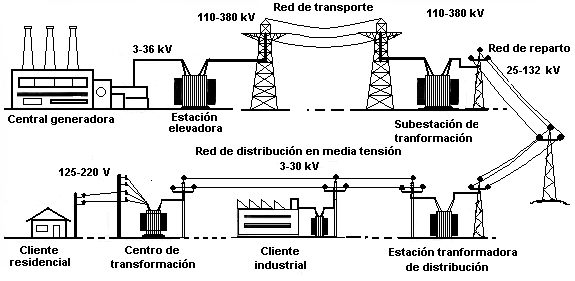
\includegraphics[width=.9\linewidth]{../figs/Redelectrica2.png}
\end{center}

\begin{itemize}
\item Generadores

\item Redes de transporte

\item Redes de distribución

\item Equipos de acondicionamiento, transformación y protección (y en
algunos casos, almacenamiento)

\item Puntos de consumo
\end{itemize}
\end{frame}


\subsection{Definición y Funciones}
\label{sec:org7a07bbf}
\begin{frame}[label={sec:orga96a8ce}]{Aparamenta}
\begin{block}{Definición}
Equipo, aparato o material previsto para ser conectado a un circuito eléctrico con el fin de asegurar una o varias de las siguientes funciones: 

\begin{itemize}
\item \alert{Protección}
\item \alert{Aislamiento}
\item \alert{Control} y \alert{Conexión}.
\end{itemize}
\end{block}
\end{frame}


\begin{frame}[label={sec:orgbab5f79}]{Protección}
\begin{itemize}
\item Protección de los \alert{elementos de los circuitos} (cables,
aparamenta) contra las tensiones térmicas y mecánicas de las
corrientes de cortocircuito.

\item Protección de las \alert{personas} en caso de producirse un defecto de
aislamiento.

\item Protección de los \alert{dispositivos y aparatos suministrados} (ej. motores).
\end{itemize}
\end{frame}

\begin{frame}[label={sec:org8e70003}]{Aislamiento}
Separar de forma verificable un circuito, un aparato o un elemento de
la planta del resto de un sistema que se encuentra en tensión, con el
fin de que el personal pueda realizar con total seguridad trabajos en
la parte aislada.
\end{frame}

\begin{frame}[label={sec:orgf5a863d}]{Control}
Modificar un sistema cargado para:

\begin{itemize}
\item Control funcional (condiciones normales de servicio, conmutación rutinaria).

\item Conmutación de emergencia (ej. seta de parada)

\item Operaciones de mantenimiento del sistema de alimentación.
\end{itemize}
\end{frame}

\begin{frame}[label={sec:org3ab2e3d}]{Arco Eléctrico}
\begin{itemize}
\item Descarga eléctrica que se forma entre dos electrodos sometidos a una
diferencia de potencial.
\end{itemize}
\begin{center}
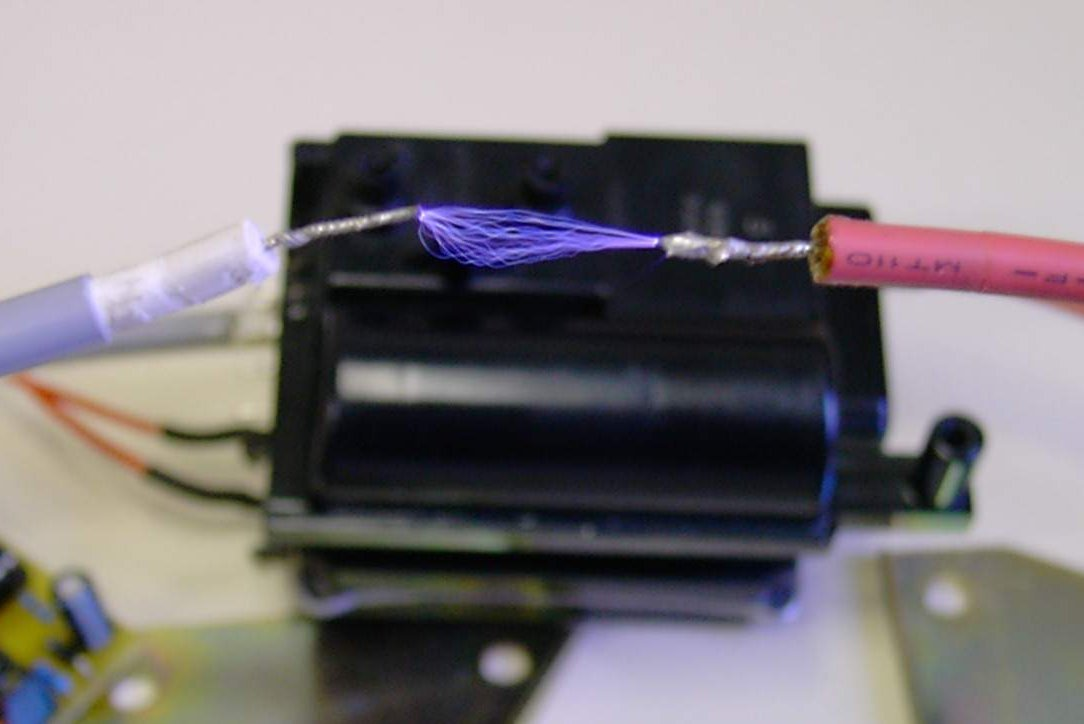
\includegraphics[height=0.35\textheight]{../figs/arco_electrico.jpg}
\end{center}

\begin{itemize}
\item Luminosidad muy intensa y un gran desprendimiento de calor (fenómeno destructivo)
\end{itemize}

\begin{block}{}
\begin{center}
Vídeo: \href{http://www.youtube.com/watch?v=WBTvGqRA4\_0}{Apertura en Alta Tensión}
\end{center}
\end{block}
\end{frame}

\begin{frame}[label={sec:org20b0ba5}]{Poder de corte y cierre}
\begin{description}
\item[{Poder de corte:}] intensidad de corriente que un dispositivo es
capaz de cortar bajo una tensión de restablecimiento determinada.

\item[{Poder de cierre:}] intensidad de corriente que un aparato es capaz
de establecer bajo una tensión dada.
\end{description}
\end{frame}

\subsection{Tipos de Dispositivos}
\label{sec:org73edabf}

\begin{frame}[label={sec:org7ca43ed}]{Seccionador}
\begin{itemize}
\item Dispositivo de dos posiciones (abierto/cerrado) enclavable y accionado manualmente que proporciona un aislamiento seguro de un circuito cuando está enclavado en la posición abierta.

\item Un seccionador no está diseñado para abrir o cerrar el paso de la corriente.
\end{itemize}

\begin{center}
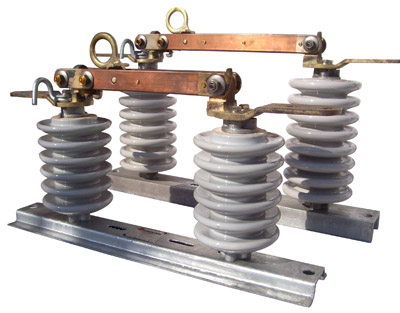
\includegraphics[height=0.6\textheight]{../figs/seccionador.jpeg}
\end{center}
\end{frame}

\begin{frame}[label={sec:org9eaf70d}]{Interruptor de carga}
\begin{itemize}
\item Dispositivo no automático (\alert{accionamiento manual}) de dos posiciones (abierto/cerrado).

\item Se utiliza para cerrar y abrir circuitos cargados en condiciones normales de circuitos sin defectos (no ofrece protección)
\end{itemize}
\begin{center}
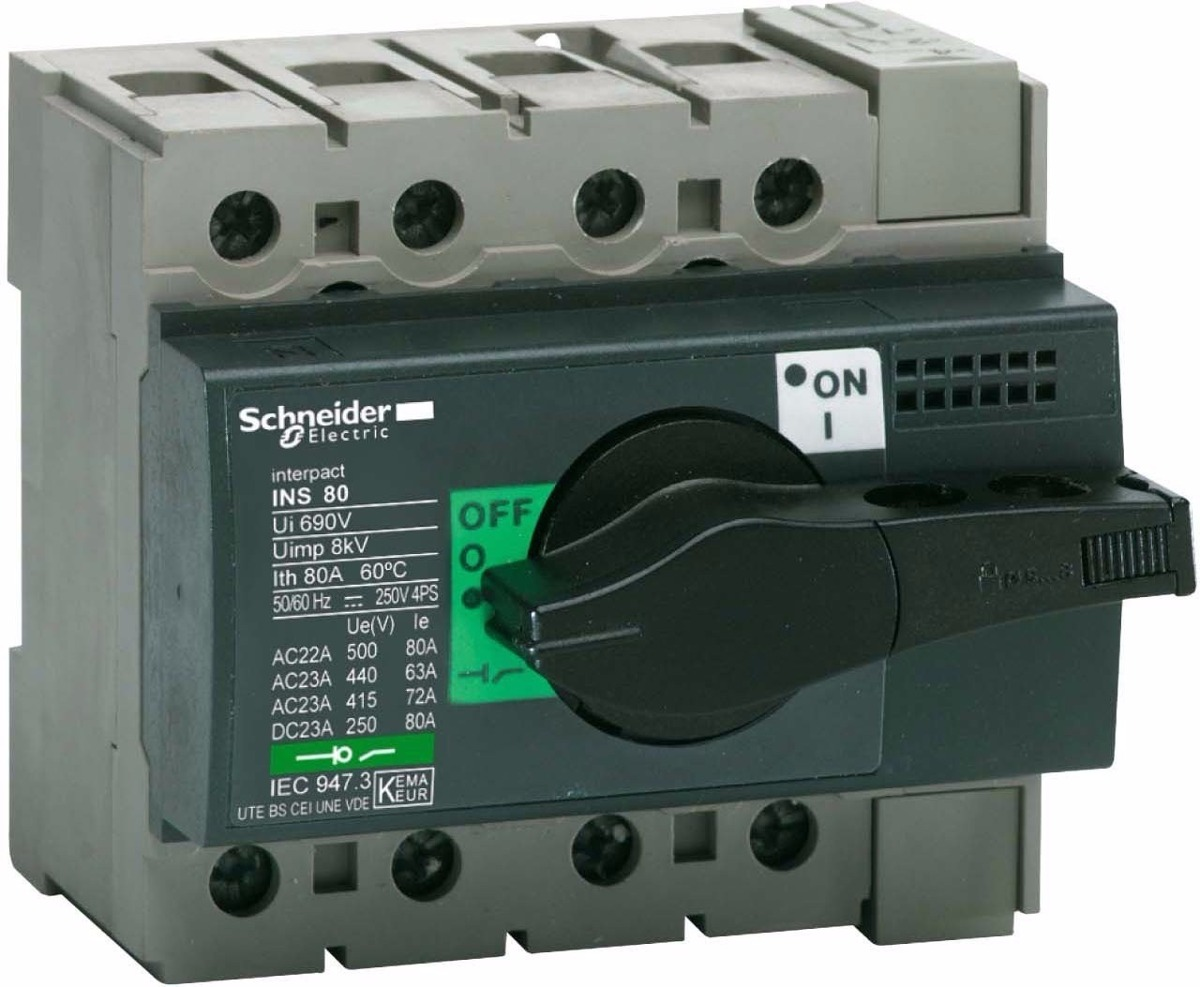
\includegraphics[height=0.6\textheight]{../figs/interruptor_manual.jpg}
\end{center}
\end{frame}


\begin{frame}[label={sec:org3474b73}]{Contactor}
\begin{itemize}
\item Dispositivo de conmutación accionado por solenoide que por lo general se mantiene cerrado mediante una corriente (reducida).

\item Se suelen controlar de forma remota por medio de pulsadores de activación/desactivación.
\end{itemize}

\begin{center}
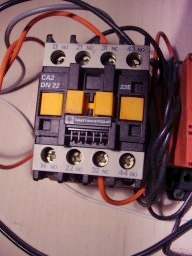
\includegraphics[height=0.6\textheight]{../figs/Contactor.jpg}
\end{center}
\end{frame}


\begin{frame}[label={sec:org382aa3d}]{Fusible}
\begin{columns}
\begin{column}{0.7\columnwidth}
\begin{itemize}
\item Se funde por Efecto Joule cuando la intensidad de corriente supera un umbral, por un cortocircuito o un exceso de carga.

\item Es capaz de abrir un circuito en carga.
\end{itemize}
\end{column}
\begin{column}{0.3\columnwidth}
\begin{center}
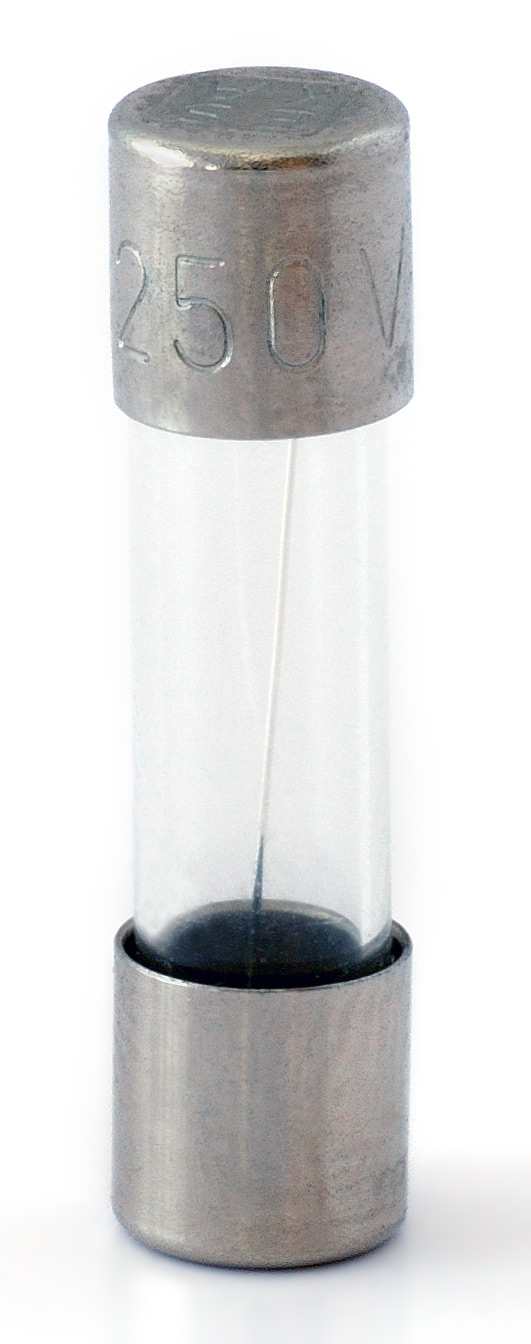
\includegraphics[width=.9\linewidth]{../figs/fusible.jpg}
\end{center}
\end{column}
\end{columns}
\end{frame}


\begin{frame}[label={sec:orgce675c7}]{Interruptor magnetotérmico}
\begin{columns}
\begin{column}{0.6\columnwidth}
\begin{itemize}
\item Dispositivo \alert{automático} capaz de interrumpir la corriente eléctrica de un circuito cuando ésta sobrepasa ciertos valores máximos.

\item Se emplea para \alert{proteger contra sobreintensidades} (\emph{efecto magnético}) y \alert{sobrecargas} (\emph{efecto Joule}).
\end{itemize}
\end{column}

\begin{column}{0.5\columnwidth}
\begin{center}
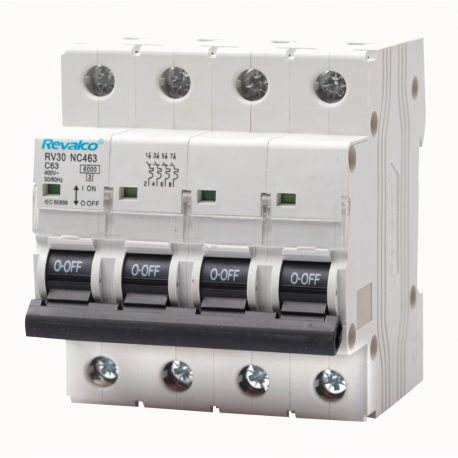
\includegraphics[width=.9\linewidth]{../figs/interruptor-magnetotermico.jpg}
\end{center}
\end{column}
\end{columns}

\begin{block}{}
Vídeo: \href{http://www.youtube.com/watch?v=c6QqnLgWbCQ}{Apertura de un PIA}
\end{block}
\end{frame}

\begin{frame}[label={sec:orge95b907}]{Interruptor diferencial}
\begin{itemize}
\item Dispositivo \alert{automático} con poder de corte ante una corriente diferencial residual (defecto de aislamiento).
\item Se emplea para la \alert{protección de las personas}.
\item Para la detección emplea un transformador toroidal que abraza a todos los conductores.
\end{itemize}

\begin{columns}
\begin{column}{0.5\columnwidth}
\begin{center}
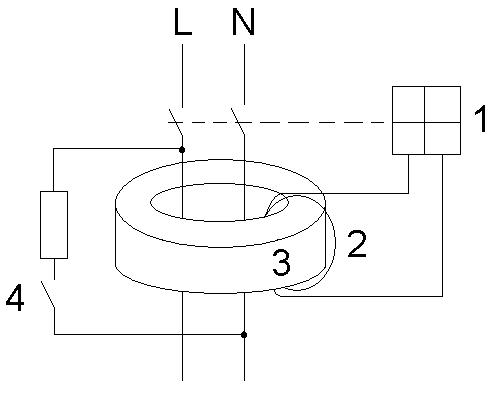
\includegraphics[width=.9\linewidth]{../figs/InterruptorDiferencial.JPG}
\end{center}
\end{column}


\begin{column}{0.5\columnwidth}
\begin{center}
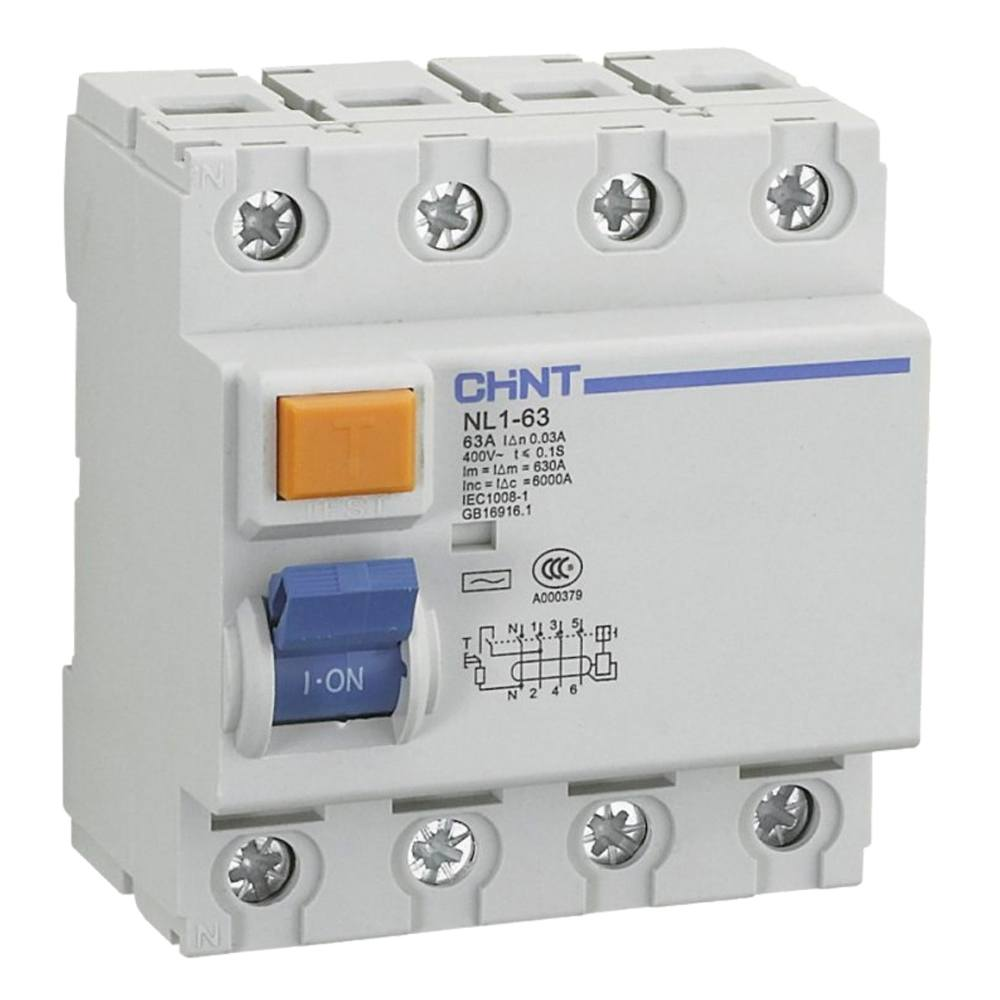
\includegraphics[width=.9\linewidth]{../figs/interruptor-diferencial.jpg}
\end{center}
\end{column}
\end{columns}
\end{frame}


\section{Recursos}
\label{sec:org446d83e}

\begin{frame}[label={sec:org0597859}]{Bibliografía}
\begin{itemize}
\item \alert{Fraile Mora, J.}: \emph{Máquinas Eléctricas}. Ed. Mc. Graw Hill.

\item \href{http://www.f2i2.net/legislacionseguridadindustrial/Si\_ambito.aspx?id\_am=76}{Reglamento Electrotécnico de Baja Tensión}

\item \href{https://www.schneider-electric.es/es/download/document/020511E10/}{Guía de diseño de instalaciones eléctricas (Schneider Electric)}

\item \href{http://www.directindustry.com/}{Equipos industriales}

\item \href{http://www.preoc.es/}{Base de Precios PREOC}
\end{itemize}
\end{frame}
\end{document}